\documentclass{article}

\usepackage[final]{neurips_data_2024}

% drop the thick/thin horizontal rules above and below the title
\makeatletter
\renewcommand{\@toptitlebar}{\vskip 0.25in \vskip -\parskip}
\renewcommand{\@bottomtitlebar}{\vskip 0.29in \vskip -\parskip \vskip 0.09in}
\makeatother

\usepackage[utf8]{inputenc}
\usepackage[T1]{fontenc}
\usepackage{hyperref}
\usepackage{url}
\usepackage{booktabs}
\usepackage{amsfonts}
\usepackage{nicefrac}
\usepackage{microtype}
\usepackage{xcolor}
\usepackage{graphicx}

\title{Section 4: Fuel Usage, Outlier Removal and Fuel Efficiency}

\author{%
  Tebogo Seopa - 2563912\\
  School of Computer Science and Applied Mathematics \\
  University of the Witwatersrand \\
  \texttt{} \\
}

\begin{document}

\maketitle

\begin{abstract}
This section covers outlier removal for the five most common currencies in the fuel
logbook dataset (Section 4.1) and six of the fuel efficiency questions that follow
from it (Section 4.2, questions 1, 2, 3, 4, 8 and 9). All figures and statistics below
are computed on the full, cleaned dataset of 1{,}173{,}702 fuelling records produced by
Sections 1--3.
\end{abstract}

\section{Outlier Removal}
\label{sec:4.1}

\subsection{Top 5 currencies by transaction count}
\label{sec:4.1.1}

The five most common currencies by number of transactions are \texttt{\$} (USD),
\texttt{£} (GBP), \texttt{€} (EUR), \texttt{CA\$} (CAD) and \texttt{R} (ZAR), as shown in
Table~\ref{tab:top5}. As anticipated in the assignment brief, the Rand is the fifth most
common currency.

\begin{table}[h]
  \caption{Top 5 currencies by transaction count.}
  \label{tab:top5}
  \centering
  \begin{tabular}{lr}
    \toprule
    Currency & Transactions \\
    \midrule
    \texttt{\$} (USD) & 741{,}655 \\
    \texttt{£} (GBP) & 87{,}554 \\
    \texttt{€} (EUR) & 59{,}254 \\
    \texttt{CA\$} (CAD) & 46{,}814 \\
    \texttt{R} (ZAR) & 36{,}388 \\
    \bottomrule
  \end{tabular}
\end{table}

\subsection{Per-currency outlier removal}
\label{sec:4.1.2}

The brief's own example, a South African user tagged with \texttt{\$} reporting
several hundred dollars for only a few tens of litres, is really a \emph{cost-per-litre
sanity check}: a fill-up's implied price (\texttt{total\_spent / litres}) has to sit
within the historically plausible retail fuel price band for that currency. Values
wildly outside that band point either to a data-entry error (stray digits, a decimal
point in the wrong place) or a currency tag that does not match the price actually paid.

For each of the top 5 currencies, a row is kept only if:
\begin{enumerate}
  \item \texttt{total\_spent} and \texttt{litres} are present and \texttt{total\_spent} $> 0$;
  \item \texttt{litres} falls in $[1, 300]$: below 1\,L is not a real fill-up, and
    300\,L comfortably covers even large trucks and vans, so this only removes clear
    entry errors (e.g. an odometer reading captured in the gallons field);
  \item the derived cost per litre falls inside a currency-specific plausible band,
    chosen generously to span 2005--2022 retail prices, including the 2021/22 price
    spike, while still excluding gross misclassifications (Table~\ref{tab:bounds}).
\end{enumerate}

These bounds were checked against the empirical percentiles of each currency: in every
case the 95th/99th percentile sits comfortably inside the band, while the 99.9th
percentile jumps by one to two orders of magnitude: a clear break between genuine
price variation and garbage data.

\begin{table}[h]
  \caption{Plausible cost-per-litre bounds used for outlier removal (local currency per litre).}
  \label{tab:bounds}
  \centering
  \begin{tabular}{lr}
    \toprule
    Currency & Band \\
    \midrule
    USD (\texttt{\$}) & 0.20 -- 3.00 \\
    GBP (\texttt{£}) & 0.50 -- 3.00 \\
    EUR (\texttt{€}) & 0.50 -- 3.00 \\
    CAD (\texttt{CA\$}) & 0.50 -- 2.50 \\
    ZAR (\texttt{R}) & 6.00 -- 24.00 \\
    \bottomrule
  \end{tabular}
\end{table}

\begin{figure}[h]
  \centering
  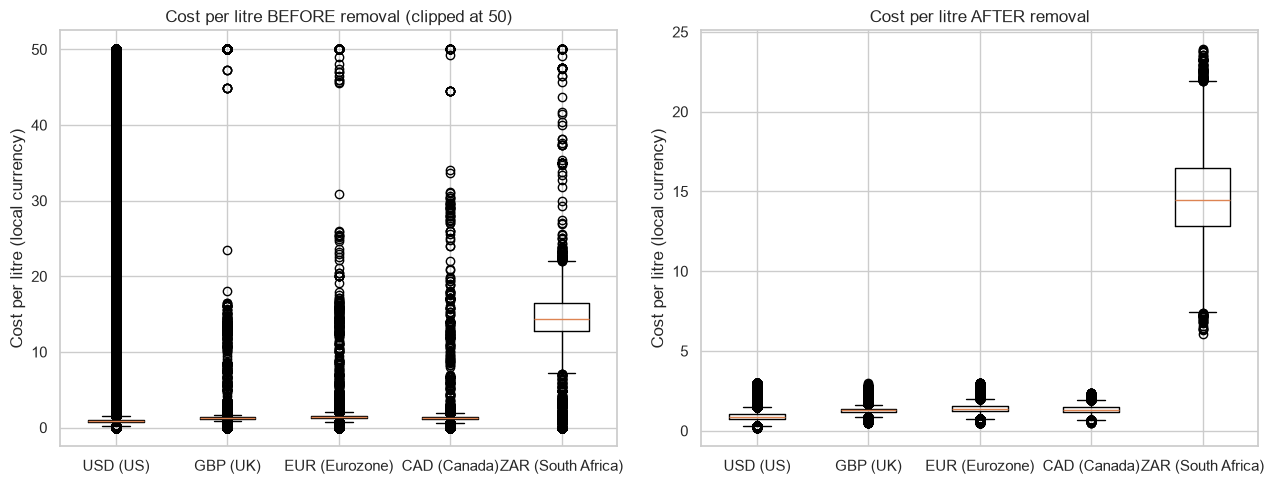
\includegraphics[width=\textwidth]{cell59_img1.png}
  \caption{Cost per litre per currency before (left) and after (right) outlier removal.
  The pre-removal panel is clipped at 50 for legibility; the uncapped tail reaches
  several orders of magnitude higher.}
  \label{fig:before_after}
\end{figure}

\subsection{Rows removed}
\label{sec:4.1.3}

Table~\ref{tab:removed} shows the number of rows removed per currency. In total,
55{,}759 of 971{,}665 rows (5.74\%) across the top 5 currencies were removed as
outliers, leaving 915{,}906 clean rows for the fuel efficiency analysis in
Section~\ref{sec:4.2}. Removal rates range from 3.03\% (CAD) to 6.32\% (USD), low
enough that the bounds are not simply discarding genuine variation, and consistent
across currencies, which suggests the bands in Table~\ref{tab:bounds} are reasonably
well calibrated rather than arbitrarily strict for any one currency.

\begin{table}[h]
  \caption{Rows removed per currency.}
  \label{tab:removed}
  \centering
  \begin{tabular}{lrrr}
    \toprule
    Currency & Before & Removed & \% removed \\
    \midrule
    USD (US) & 741{,}655 & 46{,}903 & 6.32 \\
    GBP (UK) & 87{,}554 & 4{,}031 & 4.60 \\
    EUR (Eurozone) & 59{,}254 & 2{,}201 & 3.71 \\
    CAD (Canada) & 46{,}814 & 1{,}420 & 3.03 \\
    ZAR (South Africa) & 36{,}388 & 1{,}204 & 3.31 \\
    \midrule
    \textbf{Total} & \textbf{971{,}665} & \textbf{55{,}759} & \textbf{5.74} \\
    \bottomrule
  \end{tabular}
\end{table}

\clearpage
\section{Fuel Efficiency}
\label{sec:4.2}

All analysis in this section uses the 915{,}906-row dataset remaining after the outlier
removal described in Section~\ref{sec:4.1}.

\subsection{Q1: Cost per litre per country, January 2022, converted to ZAR}
\label{sec:4.2.1}

Average January-2022 exchange rates to ZAR were computed from Nedbank's published daily
rates for the 21 trading days in January 2022 (USD/ZAR, GBP/ZAR and EUR/ZAR); CAD/ZAR
was derived as USD/ZAR $\div$ USD/CAD, using a USD/CAD rate of 1.263 sourced from
valutafx.com and ofx.com for the same month (Table~\ref{tab:fx}).

\begin{table}[h]
  \caption{Exchange rates to ZAR used for Q1 (average, January 2022).}
  \label{tab:fx}
  \centering
  \begin{tabular}{lll}
    \toprule
    Pair & Rate (1 unit = X ZAR) & Source \\
    \midrule
    USD/ZAR & 15.53 & Nedbank daily rates, 3--31 Jan 2022 (21 trading days) \\
    GBP/ZAR & 21.06 & Same source \\
    EUR/ZAR & 17.59 & Same source \\
    CAD/ZAR & 12.30 & Derived: USD/ZAR $\div$ USD/CAD (USD/CAD $\approx$ 1.263) \\
    ZAR/ZAR & 1.00 & Identity \\
    \bottomrule
  \end{tabular}
\end{table}

\begin{table}[h]
  \caption{Average cost per litre, January 2022, converted to ZAR.}
  \label{tab:q1}
  \centering
  \begin{tabular}{lrrr}
    \toprule
    Country & $n$ & Local mean & ZAR per litre \\
    \midrule
    United Kingdom (GBP) & 1{,}113 & 1.481 & 31.20 \\
    Eurozone (EUR) & 1{,}243 & 1.586 & 27.91 \\
    South Africa (ZAR) & 990 & 18.951 & 18.95 \\
    Canada (CAD) & 1{,}782 & 1.473 & 18.11 \\
    United States (USD) & 36{,}620 & 0.951 & 14.78 \\
    \bottomrule
  \end{tabular}
\end{table}

The UK and Eurozone show the highest ZAR-equivalent litre price, South Africa and Canada
sit in the middle, and the US is the cheapest. This tracks fuel taxation rather than
crude oil cost: US federal and state fuel tax is comparatively low, while UK and EU fuel
duty and VAT are among the highest in the world. South Africa's price sits above the
US/Canada level mainly because of the weaker Rand and the fuel levy and Road Accident
Fund levy stacked on the base price, not because crude is more expensive there.

\subsection{Q2: Detecting missed (unlogged) fill-ups}
\label{sec:4.2.2}

\textbf{Rule.} For a given user, fill-ups are sorted by date and the odometer gap
between consecutive logged entries is computed. If every fill-up were logged, that gap
should be reasonably close to the user's own \emph{typical} refuelling distance. A gap
much larger than that user's own median gap means at least one fill-up in between almost
certainly went unlogged. Comparing each gap to the same user's own median, rather than a
single global threshold, automatically accounts for the fact that different people drive
very different annual distances. Users need at least 3 valid gaps for their median to be
meaningful. A gap $>2\times$ that user's median gap is flagged as a likely missed
fill-up.

Plotting the ratio of each gap to that user's own median gap gives a distribution
heavily concentrated just above 1.0 (most fill-ups happen close to a driver's usual
rhythm), with a long right tail past the 2.0x threshold rather than a second, separate
peak, so the cutoff is a judgement call rather than a natural break in the data. Of
681{,}449 evaluated fill-up gaps, 120{,}248 (17.65\%) exceed twice that user's median
gap and are flagged as containing at least one missed fill-up. As a sensitivity check,
11.92\% of gaps exceed a 2.5x threshold and 7.99\% exceed 3.0x. Roughly 1 in 6
consecutive fill-up pairs shows a gap more than double that driver's usual refuelling
distance, i.e. a fill-up almost certainly happened in between without being logged.
This is a lower bound: a user who misses two fill-ups in a row, or who fills up
partially every time, will not necessarily clear a 2x threshold.

\subsection{Q3: Average distance per tank, per country}
\label{sec:4.2.3}

\begin{table}[h]
  \caption{Average distance per tank (km) by country.}
  \label{tab:q3}
  \centering
  \begin{tabular}{lrr}
    \toprule
    Country & Mean (km) & Median (km) \\
    \midrule
    Eurozone (EUR) & 593.3 & 574.3 \\
    United Kingdom (GBP) & 577.2 & 553.2 \\
    South Africa (ZAR) & 541.2 & 523.0 \\
    United States (USD) & 458.5 & 444.3 \\
    Canada (CAD) & 441.6 & 426.9 \\
    \bottomrule
  \end{tabular}
\end{table}

The Eurozone has the largest average distance per tank (593\,km). Eurozone and UK
drivers lead, ahead of South Africa, with the US and Canada lowest. This lines up with
vehicle mix rather than tank size: Europe and the UK have a much higher share of diesel
vehicles, which are materially more fuel-efficient per litre than the petrol-dominant
US/Canadian fleets, so a similarly-sized tank simply carries those vehicles further.

\subsection{Q4: Do newer vehicles drive further between fill-ups?}
\label{sec:4.2.4}

Yes: distance per tank falls steadily and close to monotonically with vehicle age
(correlation $=-0.176$), from approximately 510\,km for cars 0--3 years old down to
approximately 376\,km for cars over 25 years old, across every age bracket tested in
between. This is consistent with newer vehicles generally having better fuel
efficiency and often larger tanks, and with older vehicles losing some efficiency (wear,
outdated engine technology) over time.

\subsection{Q8: Correlation between fuel efficiency and other features}
\label{sec:4.2.8}

Fuel efficiency (\texttt{litres\_per\_100km}) is itself computed as
\texttt{litres / killometre * 100}, so \texttt{litres}, \texttt{total\_spent} and
\texttt{cost\_per\_gallon} are excluded from this analysis: correlating a value
against a term used to derive it is not a genuine relationship, it is circular. The real
candidates are distance (\texttt{killometre}), vehicle age/year, and vehicle model/make.

\texttt{car\_model} (1{,}945 levels) and \texttt{car\_make} (29 levels) are not numeric,
so each is converted to a numeric signal via 5-fold mean-target encoding: a row's
encoded value is the average efficiency of \emph{other} rows sharing its model or make,
never its own. This keeps the categorical relationship usable without a row leaking into
its own encoded value.

\begin{figure}[h]
  \centering
  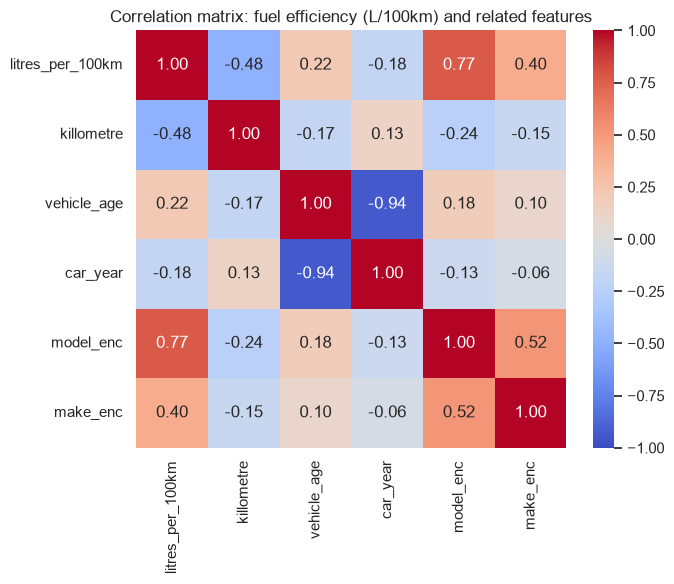
\includegraphics[width=0.6\textwidth]{cell77_img7.png}
  \caption{Correlation matrix: fuel efficiency (L/100km) and related features.}
  \label{fig:q8}
\end{figure}

This confirms the expected pattern: model (0.77) is the strongest correlate by far,
distance travelled is next ($-0.48$; more distance per tank implies a more efficient or
larger-tanked car), make is moderate (0.40), and vehicle age is weaker (0.22).
\texttt{car\_year} and \texttt{vehicle\_age} are almost perfectly anti-correlated
($-0.94$), since \texttt{vehicle\_age = fueling\_year - car\_year} and
\texttt{fueling\_year} varies far less than \texttt{car\_year}: the two columns carry
almost the same information twice.

\subsection{Q9: Random Forest feature importance}
\label{sec:4.2.9}

A Random Forest was trained on a 200{,}000-row sample using the same five
numeric/encoded features as Q8, excluding \texttt{litres\_per\_100km}'s own algebraic
inputs for the same reason as above (train $R^2 = 0.783$).

\begin{figure}[h]
  \centering
  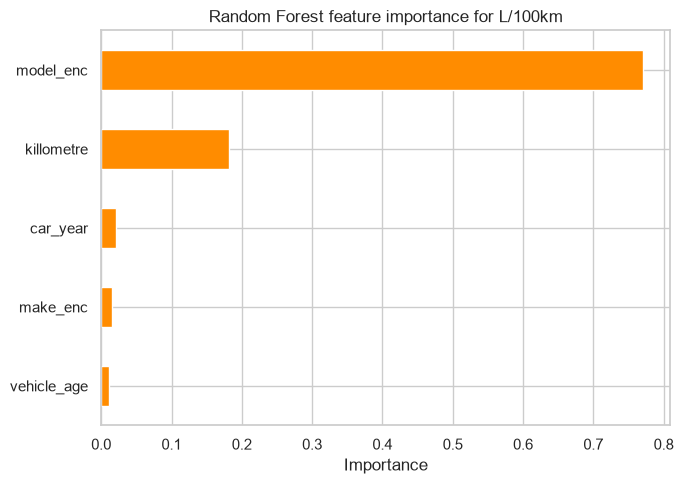
\includegraphics[width=0.6\textwidth]{cell80_img8.png}
  \caption{Random Forest feature importance for L/100km.}
  \label{fig:q9}
\end{figure}

The Random Forest agrees with the correlation ranking on the top feature: model
dominates (importance $\approx 0.77$), though it diverges further down. Distance keeps a
clear second place (importance $\approx 0.18$), much as its correlation magnitude
suggested. \texttt{car\_year}, \texttt{make\_enc} and \texttt{vehicle\_age} all drop to
under 0.02 each, well below what their correlation coefficients ($-0.18$, $0.40$,
$0.22$) would suggest on their own. Two things explain the gap. First,
\texttt{car\_year} and \texttt{vehicle\_age} are almost perfectly collinear, so the
forest can use either one and importance gets split between them rather than credited
fully to one. Second, \texttt{make\_enc} is itself largely explained by
\texttt{model\_enc} (0.52 correlation between the two, since make is a coarser version
of model), so once the forest has split on model there is little independent signal left
in make. Correlation looks at each feature in isolation; the Random Forest looks at
marginal contribution once the other features are already in the tree, so
redundant/collinear features naturally look far less important there even if their raw
correlation is moderate.

\end{document}
